%%%%%%%%%%%%%%%%%%%%%%%%%%%%%%%%%%%%%%%%%%%%%%%%%%%%%%%%%%%%%%%%%%%%%%%%%%%%%%%%%%
\begin{frame}[fragile]\frametitle{}
\begin{center}
{\Large Building Neo4j Applications with Python}

{\tiny (Ref: based on Graph Academy course, with same name)}
\end{center}
\end{frame}

%%%%%%%%%%%%%%%%%%%%%%%%%%%%%%%%%%%%%%%%%%%%%%%%%%%%%%%%%%%%%%%%%%%%%%%%%%%%%%%%%%
\begin{frame}\frametitle{Project Setup}
\begin{itemize}
\item Python version 3.9
\item A web server has been built with Flask
	\begin{itemize}
	\item Authentication is handled with JWT Tokens and Flask-JWT-Extended
	\item Passwords are encrypted and verified with bcrypt
	\item Testing is performed using pytest
	\end{itemize}
\end{itemize}

\end{frame}

%%%%%%%%%%%%%%%%%%%%%%%%%%%%%%%%%%%%%%%%%%%%%%%%%%%%%%%%%%%%%%%%%%%%%%%%%%%%%%%%%%
\begin{frame}[fragile]\frametitle{Project Setup}
\begin{itemize}
\item \lstinline|conda create -n neo4j python=3.9|
\item \lstinline|activate neo4j|
\item  Clone  the \lstinline|neo4j-graphacademy/app-python| repository from Github.
\item \lstinline|pip install -r requirements.txt|
\item Set ENV variables (list below)
\item \lstinline|python -m flask run| 
\item The REST API will listen for requests on \lstinline|http://localhost:3000|.
\end{itemize}


\begin{lstlisting}
FLASK_APP=api                       # (1)
FLASK_DEBUG=true                    # (2)
FLASK_RUN_PORT=3000                 # (3)
JWT_SECRET=secret                   # (4)
SALT_ROUNDS=10                      # (5)

NEO4J_URI=neo4j://localhost:7687    # (6)
NEO4J_USERNAME=neo4j                # (7)
NEO4J_PASSWORD=password             # (8)
\end{lstlisting}

\end{frame}

%%%%%%%%%%%%%%%%%%%%%%%%%%%%%%%%%%%%%%%%%%%%%%%%%%%%%%%%%%%%%%%%%%%%%%%%%%%%%%%%%%
\begin{frame}[fragile]\frametitle{Project codebase}
\begin{itemize}
\item \lstinline|example/| - Example code for working with the driver.
\item \lstinline|api/| - The application code:
	\begin{itemize}
	\item \lstinline|dao/| - Data Access Objects which will be modified to communicate with Neo4j
	\item \lstinline|middleware/| - Some custom middleware functions that are used by Flask throughout the request lifecycle
	\item \lstinline|routes/| - Route handlers that are registered on the server. You shouldn’t need to edit these files.
	\end{itemize}
\item \lstinline|public/| - Minified build files for the SPA. Do not edit these files.
\end{itemize}

\end{frame}

%%%%%%%%%%%%%%%%%%%%%%%%%%%%%%%%%%%%%%%%%%%%%%%%%%%%%%%%%%%%%%%%%%%%%%%%%%%%%%%%%%
\begin{frame}[fragile]\frametitle{Neo4j Sandbox}
\begin{itemize}
\item Neo4j Sandbox is a free service that allows you to create pre-populated Neo4j instances completely free of charge. Neo4j Sandbox is the perfect environment for experimenting with Neo4j.
\item You can log into Neo4j Sandbox and create a database with a number of pre-populated datasets by visiting sandbox.neo4j.com.
\item Once instance is allocated, find out, your own details (like, below)
\item Setup Env variables (like below)
\end{itemize}

\begin{lstlisting}
Browser URL https://f90e51c12eac1e9e4b512839c22ae73b.neo4jsandbox.com/browser/
Bolt URI bolt://44.200.241.114:7687
Username neo4j
Password counts-trees-tubes

NEO4J_URI=bolt://44.200.241.114:7687
NEO4J_USERNAME=neo4j
NEO4J_PASSWORD=counts-trees-tubes
\end{lstlisting}

\end{frame}

%%%%%%%%%%%%%%%%%%%%%%%%%%%%%%%%%%%%%%%%%%%%%%%%%%%%%%%%%%%%%%%%%%%%%%%%%%%%%%%%%%
\begin{frame}[fragile]\frametitle{Neo4j Python Driver}
\begin{itemize}
\item To execute a Cypher statement against a Neo4j database you will use an object called a Driver.
\item The Driver object is a thread-safe, application-wide fixture from which all Neo4j interaction derives.
\item The Driver API is topology independent, so you can run the same code against a Neo4j cluster or a single DBMS.
\item To connect to and query Neo4j from within a Python application, you use the Neo4j Python Driver.
\item You should create a single instance of the Driver in your application per Neo4j cluster or DBMS, which can then be shared across your application.
\end{itemize}

\end{frame}

%%%%%%%%%%%%%%%%%%%%%%%%%%%%%%%%%%%%%%%%%%%%%%%%%%%%%%%%%%%%%%%%%%%%%%%%%%%%%%%%%%
\begin{frame}[fragile]\frametitle{Installing the Driver}
\begin{itemize}
\item \lstinline|pip install neo4j|
\item Each driver instance will connect to one DBMS, or Neo4j cluster, depending on the value provided in the connection string.
\item The neo4j package exports a GraphDatabase object. This object provides a driver() function for creating a new driver instance.python
\end{itemize}

\begin{lstlisting}
from neo4j import GraphDatabase
driver = GraphDatabase.driver("neo4j://localhost:7687",
    auth=("neo4j", "neo"))
driver.verify_connectivity()
\end{lstlisting}

\begin{center}
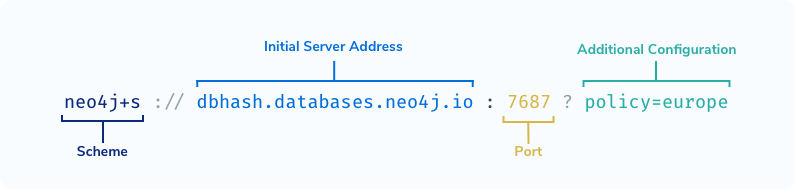
\includegraphics[width=0.8\linewidth,keepaspectratio]{neo4j87}
\end{center}	  

\end{frame}

%%%%%%%%%%%%%%%%%%%%%%%%%%%%%%%%%%%%%%%%%%%%%%%%%%%%%%%%%%%%%%%%%%%%%%%%%%%%%%%%%%
\begin{frame}[fragile]\frametitle{Choosing your Scheme}
\begin{itemize}
\item \lstinline|neo4j| - Creates an unencrypted connection to the DBMS. If you are connecting to a local DBMS or have not explicitly turned on encryption then this is most likely the option you are looking for.
\item \lstinline|neo4j+s| - Creates an encrypted connection to the DBMS. The driver will verify the authenticity of the certificate and fail to verify connectivity if there is a problem with the certificate.
\item \lstinline|neo4j+ssc| - Creates an encrypted connection to the DBMS, but will not attempt to verify the authenticity of the certificate.
\end{itemize}

Variations of the bolt scheme can be used to connect directly to a single DBMS
\begin{itemize}
\item \lstinline|bolt| - Creates an unencrypted connection directly to a single DBMS.
\item \lstinline|bolt+s| - Creates an encrypted connection directly to a single DBMS and verify the certificate.
\item \lstinline|bolt+ssc| - Creates an encrypted connection to directly to a single DBMS but will not attempt to verify the authenticity of the certificate.
\end{itemize}
\end{frame}

%%%%%%%%%%%%%%%%%%%%%%%%%%%%%%%%%%%%%%%%%%%%%%%%%%%%%%%%%%%%%%%%%%%%%%%%%%%%%%%%%%
\begin{frame}[fragile]\frametitle{What happens next?}
\begin{itemize}
\item The driver will attempt to connect to the DBMS using the supplied credentials. If everything is successful, the driver will then communicate with the DBMS and figure out the best way to execute each query.
\item You do not need to do any additional configuration when connecting to a single DBMS or a Neo4j cluster. This means you do not have to adapt your application code, regardless of which environment you connect to.
\item Once the connection has been successfully made, your application can start to interact with the data in the graph.
\end{itemize}

\end{frame}

%%%%%%%%%%%%%%%%%%%%%%%%%%%%%%%%%%%%%%%%%%%%%%%%%%%%%%%%%%%%%%%%%%%%%%%%%%%%%%%%%%
\begin{frame}[fragile]\frametitle{Adding the Driver}
\begin{itemize}
\item Inside \lstinline|api/neo4j.py|, add/update following \lstinline|init_driver()| function
\item Then test with \lstinline|python -m pytest tests/01_connect_to_neo4j__test.py|
\end{itemize}

\begin{lstlisting}
def init_driver(uri, username, password):
    # Create an instance of the driver
    current_app.driver = GraphDatabase.driver(uri, auth=(username, password))

    # Verify Connectivity
    current_app.driver.verify_connectivity()

    return current_app.driver
\end{lstlisting}

\end{frame}

%%%%%%%%%%%%%%%%%%%%%%%%%%%%%%%%%%%%%%%%%%%%%%%%%%%%%%%%%%%%%%%%%%%%%%%%%%%%%%%%%%
\begin{frame}[fragile]\frametitle{Sessions}
\begin{itemize}
\item Through the Driver, we open Sessions.
\item A session is a container for a sequence of transactions. Sessions borrow connections from a pool as required and are considered lightweight and disposable.
\item To open a new session, call the session() method on the driver. \lstinline|with driver.session() as session:|
\item Through a Session, we can run one or more Transactions.
\end{itemize}

\end{frame}

%%%%%%%%%%%%%%%%%%%%%%%%%%%%%%%%%%%%%%%%%%%%%%%%%%%%%%%%%%%%%%%%%%%%%%%%%%%%%%%%%%
\begin{frame}[fragile]\frametitle{Transactions}
There are three types of transaction exposed by the driver:


\begin{itemize}
\item Auto-commit Transactions: Auto-commit transactions are a single unit of work that are immediately executed against the DBMS and acknowledged immediately. 
\item Read Transactions: to read data from Neo4j
\item Write Transactions: to write data to the database
\end{itemize}

\end{frame}


%%%%%%%%%%%%%%%%%%%%%%%%%%%%%%%%%%%%%%%%%%%%%%%%%%%%%%%%%%%%%%%%%%%%%%%%%%%%%%%%%%
\begin{frame}[fragile]\frametitle{Transactions}

\begin{lstlisting}
// Auto-commit
session.run(
    "MATCH (p:Person {name: $name}) RETURN p", # Query
    name="Tom Hanks" # Named parameters referenced
)                    # in Cypher by prefixing with a $

// Read
def get_movies(tx, title):
    return tx.run("""
        MATCH (p:Person)-[:ACTED_IN]->(m:Movie)
        WHERE m.title = $title // (1)
        RETURN p.name AS name
        LIMIT 10
    """, title=title)

// Write
# Call tx.run() to execute the query to create a Person node
def create_person(tx, name):
    return tx.run(
        "CREATE (p:Person {name: $name})",
        name=name
    )
# Execute the `create_person` "unit of work" within a write transaction
session.execute_write(create_person, name="Michael")		
\end{lstlisting}

\end{frame}


%%%%%%%%%%%%%%%%%%%%%%%%%%%%%%%%%%%%%%%%%%%%%%%%%%%%%%%%%%%%%%%%%%%%%%%%%%%%%%%%%%
\begin{frame}[fragile]\frametitle{Manually Creating Transactions}

\begin{itemize}
\item It is also possible to explicitly create a transaction object by calling the \lstinline|begin_transaction()| function on the session.
\item This method differs from the \lstinline|execute_read| and \lstinline|execute_write()| functions, in that the transaction will have to be manually committed or rolled back depending on the outcome of the unit of work.
\end{itemize}

\begin{lstlisting}
with session.begin_transaction() as tx:
    # Run queries by calling `tx.run()`	
		try:
				# Run a query
				tx.run(query, **params)

				# Commit the transaction
				tx.commit()
		except:
				# If something goes wrong in the try block,
				# then rollback the transaction
				tx.rollback()
\end{lstlisting}
				
\end{frame}

%%%%%%%%%%%%%%%%%%%%%%%%%%%%%%%%%%%%%%%%%%%%%%%%%%%%%%%%%%%%%%%%%%%%%%%%%%%%%%%%%%
\begin{frame}[fragile]\frametitle{Example}

\begin{lstlisting}
def create_person_work(tx, name):
    return tx.run("CREATE (p:Person {name: $name}) RETURN p",
        name=name).single()

def create_person(name):
    # Create a Session for the `people` database
    session = driver.session(database="people")

    # Create a node within a write transaction
    record = session.execute_write(create_person_work,
                                    name=name)

    # Get the `p` value from the first record
    person = record["p"]

    # Close the session
    session.close()

    # Return the property from the node
    return person["name"]
\end{lstlisting}

\end{frame}

%%%%%%%%%%%%%%%%%%%%%%%%%%%%%%%%%%%%%%%%%%%%%%%%%%%%%%%%%%%%%%%%%%%%%%%%%%%%%%%%%%
\begin{frame}[fragile]\frametitle{Processing Results}

Here is an example query which retrieves a list of \lstinline|:Person| nodes related to a given Movie.

\begin{lstlisting}
# Unit of work
def get_actors(tx, movie): # (1)
    result = tx.run("""
        MATCH (p:Person)-[:ACTED_IN]->(:Movie {title: $title})
        RETURN p
    """, title=movie)

    # Access the `p` value from each record
    return [ record["p"] for record in result ]

# Open a Session
with driver.session() as session:
    # Run the unit of work within a Read Transaction
    actors = session.execute_read(get_actors, movie="The Green Mile") # (2)

    for record in actors:
        print(record["p"])

    session.close()
\end{lstlisting}

\end{frame}

%%%%%%%%%%%%%%%%%%%%%%%%%%%%%%%%%%%%%%%%%%%%%%%%%%%%%%%%%%%%%%%%%%%%%%%%%%%%%%%%%%
\begin{frame}[fragile]\frametitle{Single Result}

If you only expect a single record, you can use the single() method on the result to return the first record.

\begin{lstlisting}
def get_actors_single(tx, movie):
    result = tx.run("""
        MATCH (p:Person)-[:ACTED_IN]->(:Movie {title: $title})
        RETURN p
    """, title=movie)

    return result.single()
\end{lstlisting}

\end{frame}

%%%%%%%%%%%%%%%%%%%%%%%%%%%%%%%%%%%%%%%%%%%%%%%%%%%%%%%%%%%%%%%%%%%%%%%%%%%%%%%%%%
\begin{frame}[fragile]\frametitle{Value}

If you wish to extract a single value from the remaining list of results, you can use the value() method.

\begin{lstlisting}
def get_actors_values(tx, movie):
    result = tx.run("""
        MATCH (p:Person)-[r:ACTED_IN]->(m:Movie {title: $title})
        RETURN p.name AS name, m.title AS title, r.roles AS roles
    """, title=movie)

    return result.value("name", False)
    # Returns the `name` value, or False if unavailable
\end{lstlisting}

\end{frame}

%%%%%%%%%%%%%%%%%%%%%%%%%%%%%%%%%%%%%%%%%%%%%%%%%%%%%%%%%%%%%%%%%%%%%%%%%%%%%%%%%%
\begin{frame}[fragile]\frametitle{Consume}

The consume() method will consume the remainder of the results and return a Result Summary.

\begin{lstlisting}
def get_actors_consume(tx, name):
    result = tx.run("""
        MERGE (p:Person {name: $name})
        RETURN p
    """, name=name)

    info = result.consume()
		
# The time it took for the server to have the result available. (milliseconds)
print(info.result_available_after)

# The time it took for the server to consume the result. (milliseconds)
print(info.result_consumed_after)		
\end{lstlisting}

\end{frame}

%%%%%%%%%%%%%%%%%%%%%%%%%%%%%%%%%%%%%%%%%%%%%%%%%%%%%%%%%%%%%%%%%%%%%%%%%%%%%%%%%%
\begin{frame}[fragile]\frametitle{Types}

\begin{itemize}
\item There are some discrepancies between Java based types stored in the Neo4j database and native Python types.
\item Some values like strings, floats, booleans, and nulls have a direct mapping to Python types but more complex types need special handling.
\item The value assigned to the node variable will be the instance of a Node. Node is a type provided by the Neo4j Python Driver to hold the information held in Neo4j for the node.
\end{itemize}

\begin{lstlisting}
result = tx.run("""
MATCH path = (person:Person)-[actedIn:ACTED_IN]->(movie:Movie {title: $title})
RETURN path, person, actedIn, movie
""", title=movie)
for record in result:
    node = record["movie"]
print(node.id)              # (1)
print(node.labels)          # (2)
print(node.items())         # (3)
print(node["name"])
print(node.get("name", "N/A"))		
\end{lstlisting}

\end{frame}

%%%%%%%%%%%%%%%%%%%%%%%%%%%%%%%%%%%%%%%%%%%%%%%%%%%%%%%%%%%%%%%%%%%%%%%%%%%%%%%%%%
\begin{frame}[fragile]\frametitle{Types}

\begin{itemize}
\item Relationship objects are similar to a Node in that they provide the same method for accessing the internal ID and properties.
\item If you return a path of nodes and relationships, they will be returned as an instance of a Path.
\end{itemize}

\begin{lstlisting}
acted_in = record["actedIn"]

print(acted_in.id)         # (1)
print(acted_in.type)       # (2)
print(acted_in.items())    # (3)
print(acted_in["roles"])
print(acted_in.get("roles", "(Unknown)"))
print(acted_in.start_node) # (5)
print(acted_in.end_node)   # (6)

path = record["path"]

print(path.start_node)  # (1)
print(path.end_node)    # (2)
print(len(path))  # (1)
print(path.relationships)  # (1)
\end{lstlisting}

\end{frame}


%%%%%%%%%%%%%%%%%%%%%%%%%%%%%%%%%%%%%%%%%%%%%%%%%%%%%%%%%%%%%%%%%%%%%%%%%%%%%%%%%%
\begin{frame}[fragile]\frametitle{Temporal Data Types}

\begin{center}
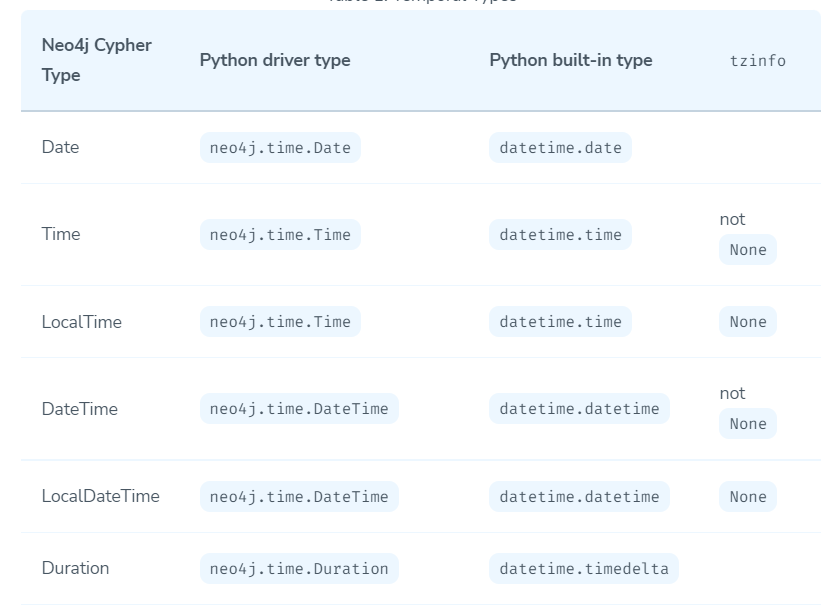
\includegraphics[width=0.4\linewidth,keepaspectratio]{neo4j88}
\end{center}	

\begin{lstlisting}
# Create a DateTime instance using individual values
datetime = neo4j.time.DateTime(year, month, day, hour, minute, second, nanosecond)

#  Create a DateTime  a time stamp (seconds since unix epoch).
from_timestamp = neo4j.time.DateTime(1609459200000) # 2021-01-01

# Get the current date and time.
now = neo4j.time.DateTime.now()

print(now.year) # 2022
\end{lstlisting}
\end{frame}

%%%%%%%%%%%%%%%%%%%%%%%%%%%%%%%%%%%%%%%%%%%%%%%%%%%%%%%%%%%%%%%%%%%%%%%%%%%%%%%%%%
\begin{frame}[fragile]\frametitle{Spatial Data Types}

\begin{itemize}
\item Cypher has built-in support for handling spatial values (points), and the underlying database supports storing these point values as properties on nodes and relationships.
\item A Cartesian Point can be created in Cypher by supplying x and y values to the point() function. The optional z value represents the height.
\item A WGS84 Point can be created in Cypher by supplying latitude and longitude values to the point() function.
\item When using the distance() function in Cypher, the distance calculated between two points is returned as a float.
\end{itemize}

\begin{lstlisting}

WITH point({x: 1, y:1}) AS one,
     point({x: 10, y: 10}) AS two

RETURN distance(one, two) // 12.727922061357855
\end{lstlisting}

\end{frame}